\documentclass[12pt]{article}

\usepackage[a4paper,margin=2cm]{geometry}

\usepackage{amsmath}
\usepackage{amssymb}
\usepackage{mathtools}

\usepackage{listings}

\usepackage{booktabs} % For tables
\usepackage[table,xcdraw]{xcolor} % For tables

\usepackage{enumerate}
\usepackage{enumitem}

\usepackage{nameref}

\usepackage{xcolor}

\definecolor{codegreen}{rgb}{0,0.6,0}
\definecolor{codegray}{rgb}{0.5,0.5,0.5}
\definecolor{codepurple}{rgb}{0.58,0,0.82}
\definecolor{backcolour}{rgb}{0.95,0.95,0.92}

\lstdefinestyle{mystyle}{
    backgroundcolor=\color{backcolour},
    commentstyle=\color{codegreen},
    keywordstyle=\color{magenta},
    numberstyle=\tiny\color{codegray},
    stringstyle=\color{codepurple},
    basicstyle=\ttfamily\footnotesize,
    breakatwhitespace=false,
    breaklines=true,
    captionpos=b,
    keepspaces=true,
    numbers=left,
    numbersep=5pt,
    showspaces=false,
    showstringspaces=false,
    showtabs=false,
    tabsize=2
}

\lstset{style=mystyle}

\DeclarePairedDelimiter\abs{\lvert}{\rvert}
\DeclarePairedDelimiter\Abs{\lVert}{\rVert}

\usepackage{fancyhdr}

\pagestyle{fancy}
\lhead{\today}
\chead{Exercise 02\\Algorithmic Foundations of Data Science}
\rhead{Fabian Grob\\Simon Michau\\Til Mohr}

\setlength{\headheight}{50pt}

\begin{document}

\section*{Exercise 1}
See \refname{appendix} for code.
\begin{center}
	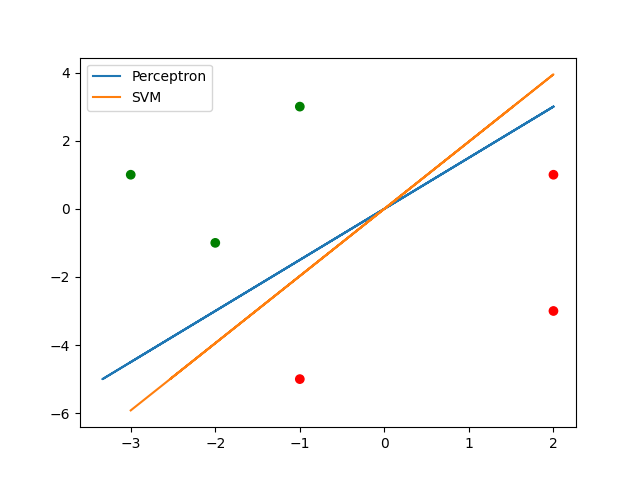
\includegraphics{code/exercise_01.png}
\end{center}
\begin{enumerate}[label=(\alph*)]
	\item	Perceptron Learning: \\
			\bigskip

			Updating vector $w=(0, 0)$ using $(x,y)=((2, 1), -1)$ \\
			$w=(-2, -1) \rightarrow w=(0, 0) + y=-1 * x=(2, 1)$ \\
			\bigskip

			Updating vector $w=(-2, -1)$ using $(x,y)=((-1, 3), 1)$ \\
			$w=(-3, 2) \rightarrow w=(-2, -1) + y=1 * x=(-1, 3)$ \\
			\bigskip

			Margin ($\underset{(x,y)\in S}{\text{min}} \frac{|\langle w,x \rangle|}{|| w ||}$): $1.1094003924504583$
	\item	SVM Learning: \\
			\bigskip

			$w^*: (-0.6074814098863559, 0.30790724037405226)$ \\
			Margin ($\underset{(x,y)\in S}{\text{min}} \frac{|\langle w,x \rangle|}{|| w ||}$): $1.331824259573374$
\end{enumerate}


\section*{Exercise 2}
\begin{enumerate}[label=(\alph*)]
	\item	$\hat{w}=\textbf{1}=(1, \dots, 1) \in \{1\}^n$ is a suitable weight vector, since $\langle \hat{w},x \rangle$ is only positive, iff $x$ contains more $1$'s than $-1$'s.
	\item	$\lambda = n$, since $\Abs{x}$ is maximum when $x$ consists of either only $1$'s or only $-1$'s. \\
			$\gamma = \frac{1}{n}$ since the margin is minimal for a $x$ which consists of an by one number off amount of $1$'s and $-1'$. Thus, $\frac{\abs{\langle w,x \rangle}}{\Abs{w}} = \frac{1}{n}$ \\
			Using Theorem 1.13 we can derive that the perceptron algorithm finds a linear separator after at most $\left(\frac{\lambda}{\gamma}\right)^2 = \left( \frac{n}{\frac{1}{n}}\right)^2 = n^4$ updates.
	\item	The smallest possible number of updates is $1$. Let $(x_1 \coloneqq (1, \dots, 1), y_1 \coloneqq 1)$ be the first element in $S$. \\
			Initially the weight vector is $w=((0, \dots, 0))$. Thus, $sgn(\langle w, x_1 \rangle) \neq y_1$ holds and we update $w \leftarrow w + y_1 x_1 = (1, \dots, 1)$. \\
			As discussed previously, this is already a suitable weight vector, therefore we do not have to update $w$ ever again.
	\item	No, we cannot. Counterexample: \\
			Let $n=3$, $x=(1,1,x_3) \in \mathbb{R}^3$. We know, that $x$ should be classified as $1$. However, for every weight vector $w = (w_1, w_2, w_3) \in \mathbb{R}^3$ we can set $x_3$ to the value of $x_3 \coloneqq -\frac{w_1 + w_2}{w_3}$ ($x_3 \coloneqq -(w_1 + w_2)$ iff $w_3 = 0$), that would lead to a false classification of $x$:
			$$sgn(\langle w,x \rangle) = sgn(w_1 + w_2 + x_3 \cdot w_3) = sgn(0) = 0 \neq 1$$
			So for every $w$ we can compute a vector $x$ so that $w$ is not consistent with $\{(x, maj(x))\}$. Thus, no such linear separator exists.
\end{enumerate}

\section*{Exercise 3}
\begin{enumerate}[label=(\alph*)]
	\item	\[\tau : \mathbb{R}^2 \rightarrow \mathbb{R}^4, (x,y) \mapsto (x,y,(\sin(xy))^2, (\cos(xy))^2)\]
	\item	\[\tau' : \mathbb{R}^2 \rightarrow \mathbb{R}^3, (x,y) \mapsto (x,y, (\sin(xy))^2)\]
			We make use of $1 = (\sin(\phi))^2 + (\cos(\phi))^2$. Hence:
			\begin{align*}
				h(x,y) &= sgn(w_1 x + w_2 y + w_3 (\sin(xy))^2 + w_4 (\cos(xy))^2 - b) \\
				&= sgn(w_1 x + w_2 y + w_3 (\sin(xy))^2 + w_4 (1-(\sin(xy)))^2 - b) \\
				&= sgn(w_1 x + w_2 y + w_3 (\sin(xy))^2 + w_4 - w_4 (\sin(xy))^2 - b) \\
				&= sgn(w_1 x + w_2 y + (w_3 + w_4) \cdot (\sin(xy))^2 - (b - w_4)) \\
				&= sgn(w_1 x + w_2 y + w_3' \cdot (\sin(xy))^2 - b') \\
				&\eqqcolon h'(x,y)
			\end{align*}
			where $w_3' \coloneqq w_3 + w_4$ and $b' \coloneqq b - w_4$.
\end{enumerate}

\section*{Exercise 4}
See \refname{appendix} for code.
\begin{enumerate}[label=(\alph*)]
	\item	Clusters: [[], [], []] \\
			Centres: [(-3, 5), (-2, 4), (-1, 2)] \\

			Clusters: [[(-3, 5)], [(-2, 4)], [(-1, 2), (-4, 0), (1, -2), (2, 0), (2, 1), (3, 5)]] \\
			Centres: [(-3.0, 5.0), (-2.0, 4.0), (0.5, 1.0)] \\

			Clusters: [[(-3, 5)], [(-2, 4), (-4, 0)], [(-1, 2), (1, -2), (2, 0), (2, 1), (3, 5)]] \\
			Centres: [(-3.0, 5.0), (-3.0, 2.0), (1.4, 1.2)] \\

			Clusters: [[(-3, 5), (-2, 4)], [(-1, 2), (-4, 0)], [(1, -2), (2, 0), (2, 1), (3, 5)]] \\
			Centres: [(-2.5, 4.5), (-2.5, 1.0), (2.0, 1.0)] \\

			Final Clusters: [[(-3, 5), (-2, 4)], [(-1, 2), (-4, 0)], [(1, -2), (2, 0), (2, 1), (3, 5)]] \\
			Final Centers: [(-2.5, 4.5), (-2.5, 1.0), (2.0, 1.0)]
	\item	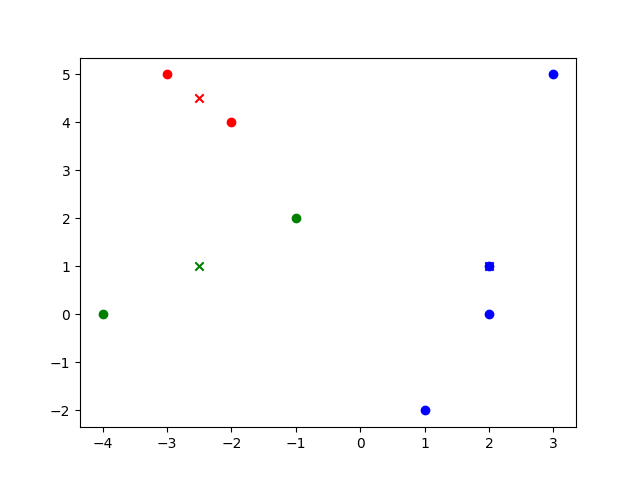
\includegraphics{code/exercise_04_a.png}
	\item	Circumcenter $c = (-0.25, 2.75)$ \\
			Line 1: $y = 2.75$ (separating red and green) \\
			Line 2: $x = -0.25$ (separating green and blue) \\
			Line 3: $y = 2.75 + \frac{x+0.25}{3.5} \cdot 0.5$ (separating red and blue)
	\item	\[z^1=x_1=(-3,5), z^2=x_8=(3,5), z^2=x_4=(-4,0)\]
			produces following clustering: \\
			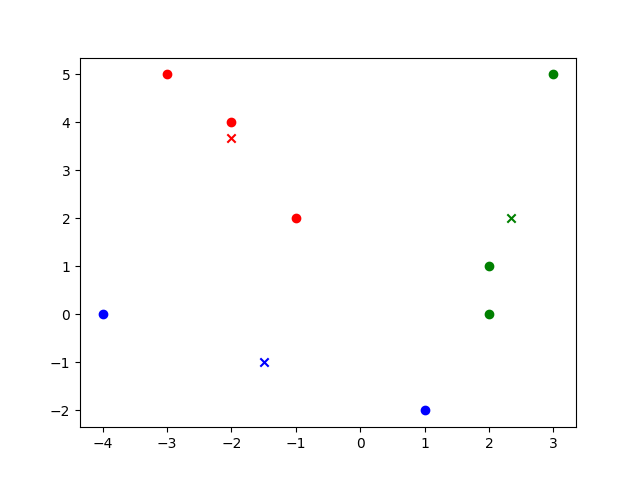
\includegraphics{code/exercise_04_d.png}
	\item	Yes, for example
			$z^1=\begin{bmatrix} -4 \\ 3 \end{bmatrix}$,
			$z^2=\begin{bmatrix} -1.5 \\ 3 \end{bmatrix}$,
			$z^3=\begin{bmatrix} 2 \\ -2 \end{bmatrix}$,
\end{enumerate}

\section*{Exercise 5}
\begin{enumerate}[label=(\alph*)]
	\item	\[\mathbb{E}[Y_n] = \mathbb{E}[\prod_{i=1}^n X_i] = \prod_{i=1}^n \mathbb{E}[X_i] = \prod_{i=1}^n 3.5 = 3.5^n\]
			\begin{align*}
				\text{Var}(Y_n) &= \mathbb{E}[(Y_n - \mathbb{E}[Y_n])^2] = \mathbb{E}[(Y_n - 3.5^n)^2] = \mathbb{E}[Y_n^2 - 2 \cdot 3.5^n \cdot Y_n + 3.5^{2n}] \\
				&= \mathbb{E}[Y_n^2] - 2 \cdot 3.5^n \cdot \mathbb{E}[Y_n] + 3.5^{2n} \\
				&= \mathbb{E}[Y_n] \cdot \mathbb{E}[Y_n] - 2 \cdot 3.5^n \cdot 3.5^n + 3.5^{2n} \\
				&= 3.5^n \cdot 3.5^n - 2 \cdot 3.5^n \cdot 3.5^n + 3.5^{2n} \\
				&= 0
			\end{align*}
	\item	\begin{enumerate}[label=(\roman*)]
				\item	\[Pr(Z_{300} \leq 10) = 1 - Pr(Z_{300} \geq 11) \geq 1 - \frac{\frac{50}{11}}{300} = 1-  \frac{65}{66} = \frac{1}{66} = 0.015\]
				\item	\[ P(|Z_{300} - E(X)| \leq 10) = P(|Z_{300} - E(X)| < 11) \geq 1 - \frac{V(X)}{11^2} = 1 - \frac{\frac{125}{3}}{11^2} = \frac{238}{363} = 0.656\]
				\item Chernoff: \[ P\left[\sum X_{i}\leq (1-\delta )\cdot pn\right]\leq \exp \left(-{\frac {\delta ^{2}}{2}}pn\right)\]
				\[\Rightarrow (1-\delta)\cdot 50 = 10 \Leftrightarrow
				1 - \delta = \frac{1}{5} \Leftrightarrow
				- \delta = -\frac{4}{5} \Leftrightarrow
				\delta = \frac{4}{5}\] \\
				\[ \Rightarrow P(X \leq 10) \leq \exp(-\frac{\frac{4}{5}^2}{2}\cdot 50) = 1.125 \cdot 10^{-7}\]
				\item \[ \Pr \left[\sum (X_{i}-{\textrm {E}}[X_{i}])\geq c\right]\leq {\textrm {exp}}\left({\frac {-2c^{2}}{\sum (b_{i}-a_{i})^{2}}}\right)\] with $a = 0 $ and $b = 1$. Centering around the mean of 50 leads to $a = -50$ and $b = -49$ and $c = 10 - 50 = -40$:\\
				\[ P(X\leq 10) = 1 - P(X\qeq 10) > 1 - \exp\left({\frac {-2(-40)^{2}}{300 \cdot (-49 + 50)^{2}}}\right) = 0.999 \]
			\end{enumerate}
			
\end{enumerate}
The best bound is given by the Chernoff inequality as the actual probability is binomially distributed with \[ P(X\leq 10) = 3.03 \cdot 10^{-13} \] with $n = 300 $ and $p = \frac{1}{6}$.

\section*{Exercise 6}
\begin{enumerate}[label=(\alph*)]
	\item	\begin{align*}
				& H(X \vert Y) + H(X) \Leftrightarrow (\sum_{y \in rg(Y)} Pr(Y=y) \left( \sum_{x \in rg(X)} Pr(X=x \vert Y=y) \cdot \log(\frac{1}{Pr(X=x \vert Y=y)} \right)) \\
				& + (\sum_{y \in rg(Y)} Pr(Y=y) \cdot \log(\frac{1}{Pr(Y=y)})) \\
				&\Leftrightarrow (\sum_{y \in rg(Y)} \sum_{x \in rg(X)} \left(  Pr(X=x, Y=y) \cdot \log(\frac{Pr(Y=y)}{Pr(X=x, Y=y)} \right)) \\
				& + (\sum_{y \in rg(Y)} Pr(Y=y) \cdot \log(\frac{1}{Pr(Y=y)})) \\
				&\Leftrightarrow (\sum_{y \in rg(Y)} \sum_{x \in rg(X)} \left( Pr(X=x, Y=y) \cdot (\log(Pr(Y=y) - \log(Pr(X=x, Y=y)) \right)) \\
				& - (\sum_{y \in rg(Y)} Pr(Y=y) \cdot \log(Pr(Y=y))) \\
				&\Leftrightarrow (\sum_{y \in rg(Y)} \sum_{x \in rg(X)} \left( Pr(X=x, Y=y) \cdot \log(Pr(Y=y)) \right)) \\
				& + (\sum_{y \in rg(Y)} \sum_{x \in rg(X)} \left( Pr(X=x, Y=y) \cdot -\log(Pr(X=x, Y=y)) \right)) \\
				& - (\sum\limits_{\substack{y \in rg(Y) \\ x \in rg(X)}} Pr(Y=y, X=x) \cdot \log(Pr(Y=y))) \\
				&\Leftrightarrow (\sum_{y \in rg(Y)} \sum_{x \in rg(X)} \left( Pr(X=x, Y=y) \cdot \log(Pr(Y=y)) \right)) \\
				& + H(X,Y) \\
				& - (\sum\limits_{\substack{y \in rg(Y) \\ x \in rg(X)}} Pr(Y=y, X=x) \cdot \log(Pr(Y=y))) \\
				&\Leftrightarrow H(X,Y)
			\end{align*}
	\item	\begin{align*}
				H(X \vert Y) &\Leftrightarrow \sum_{y \in rg(Y)} Pr(Y=y) \left( \sum_{x \in rg(X)} Pr(X=x \vert Y=y) \cdot \log(\frac{1}{Pr(X=x \vert Y=y)}) \right) \\
				&\Leftrightarrow \sum_{y \in rg(Y)} Pr(Y=y) \left( \sum_{x \in rg(X)} Pr(X=x) \cdot \log(\frac{1}{Pr(X=x)}) \right) \\
				&\Leftrightarrow \sum_{y \in rg(Y)} Pr(Y=y) \left( H(X) \right) \\
				&\Leftrightarrow H(X) \cdot \sum_{y \in rg(Y)} Pr(Y=y) \\
				&\Leftrightarrow H(X) \\
			\end{align*}
\end{enumerate}


\section*{Appendix}\label{appendix}
\subsection*{Code for Exercise 1}
\lstinputlisting[language=Python]{code/exercise_01.py}
\subsection*{Code for Exercise 4}
\lstinputlisting[language=Python]{code/exercise_04.py}

\end{document}